%  Template for ICASSP-2021 paper; to be used with:
%          spconf.sty  - ICASSP/ICIP LaTeX style file, and
%          IEEEbib.bst - IEEE bibliography style file.
% --------------------------------------------------------------------------
\documentclass{article}
\usepackage{spconf,amsmath,graphicx,hyperref}

% Example definitions.
% --------------------
\def\x{{\mathbf x}}
\def\L{{\cal L}}

% Title.
% ------
\title{AIML 425 Assignemnt 4}
%
% Single address.
% ---------------
\name{Quan Zhao (Student ID: 300471028)}
%\name{Author(s) Name(s)\thanks{Thanks to XYZ agency for funding.}}
\address{Victoria University of Wellington}


\begin{document}
%\ninept
%
\maketitle
%
\section{Introduction}
\label{sec:intro}

An autoencoder is a type of artificial neural network used primarily for unsupervised learning tasks, especially data compression and noise reduction. Its architecture is designed to learn efficient codings or representations of input data, typically for the purpose of dimensionality reduction or for learning generative models of data.
In this work, I will present my understanding of it by train an autoencoder on a 3D data that are uniformly distributed over the surface of a cube data.
and then, introducing a suitable method to control the distribution of the latent (bottleneck) variable
as well as add iid Gaussian noise to the latent (bottleneck) variable with an adjustable
(not learned) SNR.
after that, we discuss the attributes of the reconstruction that you obtain at various SNRs
and dimensionalities of the latent vector.
at last, we select a quality measure, and quantify the generative performance of your autoencoder


Intro contents \cite{domingos2012few}

\section{THEORY}
\label{sec:theory}

\subsection{Variational autoencoder (VAE)}
\label{ssec:vae}

Variational Autoencoders, commonly known as VAEs, are a type of generative model that extends traditional autoencoders by introducing probabilistic layers and a specific regularization term. Unlike standard autoencoders, which learn deterministic encodings of the input data, VAEs learn probabilistic mappings. This means that the latent space of a VAE is designed to follow a specific probability distribution, typically a Gaussian distribution.

\begin{equation}
  \text{ELBO}(\theta, \phi; x) = \text{E}_{q_\phi(z|x)}[\log p_\theta(x|z)] - \text{KL}(q_\phi(z|x) || p(z))
  \end{equation}
  

\subsection{Signal-to-Noise Ratio (SNR)}
\label{ssec:snr}

The Signal-to-Noise Ratio, commonly abbreviated as SNR, is a measure used to quantify the level of a desired signal relative to the level of background noise. 
In the context of digital signals and data processing, the SNR provides insights into the clarity and quality of a signal amidst the presence of noise.

In autoencoders, the latent or bottleneck variable captures the compressed representation of the input data. By introducing noise, specifically iid (independent and identically distributed) Gaussian noise, to this latent space, one can simulate real-world scenarios where data might be corrupted or perturbed. This process can also act as a form of regularization, potentially improving the generalization capability of the autoencoder.

Why Gaussian Noise? 
Gaussian noise, characterized by its bell-shaped probability distribution, is a common choice due to its natural occurrence in many real-world scenarios. When noise is added to the latent space of an autoencoder, it's essential that this noise doesn't dominate the original signal. The SNR can help in quantifying the balance between the latent variable's information (signal) and the introduced noise.

\subsection{Earth Mover's Distance (EMD)}
\label{ssec:emd}

The Earth Mover's Distance, commonly referred to as EMD or Wasserstein distance, is a metric that quantifies the dissimilarity between two probability distributions over a given space. Originating from the fields of transportation and economics, EMD has found extensive applications in computer vision, machine learning, and image retrieval due to its sensitivity to the spatial distribution of data points.

Imagine two distinct piles of soil representing two distributions. The goal is to reshape one pile to match the other. EMD measures the least amount of "work" required to achieve this, where "work" is determined by the product of the soil amount and the distance it's moved.

For two distributions 
$P$ and 
$Q$, EMD is the minimal cumulative cost to transfer mass from points in 
$P$ to points in 
$Q$. This transformation can be represented as a linear programming problem, though faster algorithms and approximations have been developed for specific scenarios.


\section{RESULTS}
\label{sec:results}

\subsection{Data}
\label{ssec:data}

This work is based on the data which uniformly distributed over the surface of a cube. 
The data distribution is showing in Figure $\ref{fig:data}$.

\begin{figure}[htb]
  \begin{minipage}[b]{1.0\linewidth}
    \centering
    \centerline{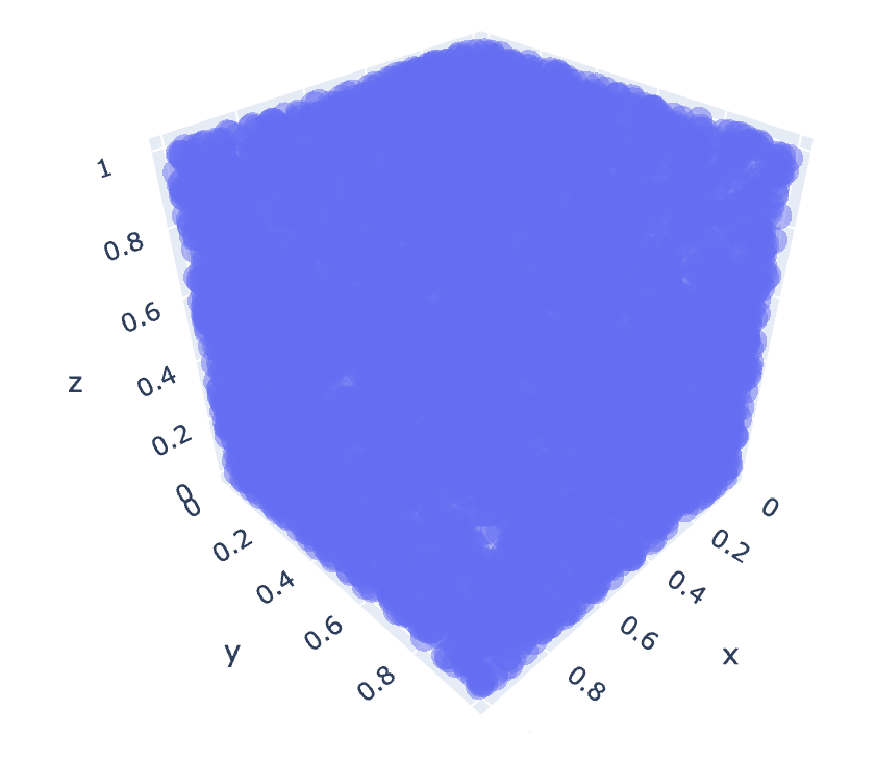
\includegraphics[width=7.0cm]{images/data}}
  \end{minipage}
  \caption{3D data that are uniformly distributed over the surface of a cube}
  \label{fig:data}
  %
  \end{figure}

\subsection{Basic autoencoder}
\label{ssec:basicautoencoder}

We train autoencoder start with basic approach with encoder and decoder and MSE as object function.
After tuning the dimension of latent variables by visualize the decoder output. 
We find the model work perty well when we set 7 latent varialbes.
But, we also found the distribution of each latent varialbe is not stable, as shows in Figure $\ref{fig:basic}$.

\begin{figure}[htb]
  \begin{minipage}[b]{1.0\linewidth}
    \centering
    \centerline{\includegraphics[width=7.0cm]{images/basic_r1}}
  %  \vspace{1.5cm}
    \centerline{(a) round 1}\medskip
  \end{minipage}
  \hfill
  \begin{minipage}[b]{1.0\linewidth}
    \centering
    \centerline{\includegraphics[width=7.0cm]{images/basic_r2}}
  %  \vspace{1.5cm}
    \centerline{(b) round 2 }\medskip
  \end{minipage}
  %
  \caption{distribution of latent variables}
  \label{fig:basic}
  %
  \end{figure}

\subsection{Control the distribution of thelatent (bottleneck) variable}
\label{ssec:VAE}


\section{CONCLUSION}
\label{sec:conclusion}


\section{STATEMENT OF ALL TOOLS USED}
\label{sec:statementofalltoolsused}

In this work, we used Pytorch geometric package to generate data, create, train models. 
The Plotly package helped us visualize in 3D. 

Source codes are published in github: 
$\href{https://github.com/felixzhao/AIML425-ASSN-3/blob/main/AIML425_Assignment_3.ipynb}{URL}$
 (runable in google colab)



% To start a new column (but not a new page) and help balance the last-page
% column length use \vfill\pagebreak.
% -------------------------------------------------------------------------
%\vfill
%\pagebreak

\vfill\pagebreak

% References should be produced using the bibtex program from suitable
% BiBTeX files (here: strings, refs, manuals). The IEEEbib.bst bibliography
% style file from IEEE produces unsorted bibliography list.
% -------------------------------------------------------------------------
\bibliographystyle{IEEEbib}
\bibliography{strings,refs}

\end{document}
